% REMEMBER: You must not plagiarise anything in your report. Be extremely careful.

\documentclass{l4proj}

% put any additional packages here
\usepackage{amsmath}
\usepackage{pdfpages}

\begin{document}

%==============================================================================
%% METADATA
\title{Level 4 Project: An Investigation into Importance of Different Geometric Components when Extending a Cross Section of Four Dimensional Objects}
\author{Joe Subbiani}
\date{March 18, 2022}

\maketitle

%==============================================================================
%% ABSTRACT
\begin{abstract}
    %Every abstract follows a similar pattern. Motivate; set aims; describe work; explain results.
    %\vskip 0.5em
    %``XYZ is bad. This project investigated ABC to determine if it was! better. ABC used XXX and YYY to implement ZZZ. This is particularly interesting as XXX and YYY have never been used together. It was found that ABC was 20\% better than XYZ, though it caused rabies in half of subjects.''

    Four dimensional space is a mathematical concept that cannot be visualised in its entirety by humans. Several paradigms exist to visualise four dimensional objects in 3D, but a viewer will only be able to see a fraction of a 4D object at one time.
    \vskip 0.5em
    Ray marching over signed distance functions provide a quick method of rendering 3D cross sections of a wide range of primitive 4D shapes.
    3D cross sections of 4D objects provides a platform to develop extended visualisations to provide a user with more information about a 4D object. Such extensions have been explored in other literature. This paper aims to evaluate the effectiveness of a series of extensions to 3D cross sections of 4D objects; each representation providing the user with more information in order to help them interpret and manipulate the object they are handling.
    \vskip 0.5em

    TODO: Results of Experiment
    It was found that ...
    
\end{abstract}

%==============================================================================
%% ACKNOWLEDGEMENTS
\renewcommand{\abstractname}{Acknowledgements}
\begin{abstract}
    I would like to thank my supervisor, Dr. John Williamson for the constant support and advice throughout the project, within and outside of the weekly meetings. Thanks to his guidance and support, I was able to take this project as far as I have, and fully explore the complexities of the fourth dimension.
\end{abstract}
%==============================================================================

% EDUCATION REUSE CONSENT FORM
% If you consent to your project being shown to future students for educational purposes then insert your name and the date below to  sign the education use form that appears in the front of the document. You must explicitly give consent if you wish to do so. If you sign, your project may be included in the Hall of Fame if it scores particularly highly.

% Please note that you are under no obligation to sign  this declaration, but doing so would help future students.

\def\consentname {Dominic Joe Subbiani} % your full name
\def\consentdate {24 January 2022} % the date you agree

\educationalconsent


%==============================================================================
\tableofcontents

%==============================================================================
%% Notes on formatting
%==============================================================================
% The first page, abstract and table of contents are numbered using Roman numerals and are not included in the page count. 

% From now on pages are numbered using Arabic numerals. Therefore, immediately after the first call to \chapter we need the call \pagenumbering{arabic} and this should be called once only in the document. 

% Do not alter the bibliography style.

% The first Chapter should then be on page 1. You are allowed 40 pages for a 40 credit project and 30 pages for a 20 credit report. This includes everything numbered in Arabic numerals (excluding front matter) up to but excluding the appendices and bibliography.

% You must not alter text size (it is currently 10pt) or alter margins or spacing.

%==================================================================================================================================

% IMPORTANT
% The chapter headings here are **suggestions**. You don't have to follow this model if it doesn't fit your project. Every project should have an introduction and conclusion, however. 

%==================================================================================================================================
\chapter{Introduction}

% reset page numbering. Don't remove this!
\pagenumbering{arabic} 

\section{The Fourth Dimension}

The world is described as three dimensional Euclidean space, conventionally referred to as $\mathbb{R}^3$. Three axes, conventionally labeled \(x\), \(y\) and \(z\), define the three degrees of translational freedom an entity can move within. All three axes that make up Euclidean space exist perpendicular to each other. Four dimensional space, conventionally referred to as $\mathbb{R}^4$, is the mathematical concept where a fourth perpendicular axes, conventionally labeled \(w\), exists perpendicular to all of the other three dimensional axes. It is impossible to visualise four dimensions in its entirety and often has to be abstracted to an analogues 3D - 2D example to reason and understand the behaviour of four dimensional entities. 

\section{Opportunities for Exploration}

Handling four dimensional space presents a number of opportunities and challenges that come with the desire to explore, interpret and manipulate higher dimensional objects. The most immediate challenge is that of being able to manipulate a four dimensional object. Rotating an object is a non trivial challenge and the most common method of rotation in 3D cannot be extended to higher dimensions. There are several ways in which users can interact with 3D objects. Another non-trivial challenge is finding intuitive ways in which a user can manipulate a 4D object through a two dimensional user interface.
\vskip 0.5em
To understand the orientation of an object, a user needs to be able to differentiate similar faces of that object from each other. Colour, patterns and textures can be applied to an object in order to assist in comprehending the current status of an object in comparison to an otherwise visually similar counterpart. An example of this is a cube rotated 90 degrees (\(\frac{\pi}{2}\) radians) and the same cube rotated by 270 degrees (\(\frac{3\pi}{2}\) radians).
\vskip 0.5em
In this paper several methods will be applied in an attempt to provide more information about a four dimensional object. Such methods include: viewing the object from other angles, attempts to visualise the object in its entirety, and abstractions of the rotation of an object in order to help understand higher dimensional rotations.

\section{Motivation}

% first, motivate then state the general problem clearly. 

Three dimensional space is very neat. There are three degrees of translational freedom expressed by the three axes \(x\), \(y\) and \(z\). There are a further three degrees of rotational freedom that are most commonly expressed as rotations about each axis. 
This supposed tidiness has lead to misconceptions that are so heavily rooted in the average persons understanding of geometry such that nearly every digital 3D system is built upon a mathematically impure foundation. 
%
In the 3D world, these misconceptions do not matter, and the mathematics is still sound. Quaternions, the most common method of controlling or interpreting rotation, is heavily used in gyroscopic devices, interactive digital 3D environments, animation and robotics. More abstract practices such as mathematics and physics, however, need to consider geometry in higher dimensional spaces.
\vskip 0.5em
A variety of fields within science and engineering utilise the visualisation of higher dimensional spaces to tackle a variety of problems. For any problem defined in \(n\) dimensional space, to understand it more intuitively, it is often suitable to reduce the dimensionality of the problem. However, when a problem is reduced to $\mathbb{R}^3$ or $\mathbb{R}^2$ it may become somewhat trivial. Visualisation of 4D objects can often server as the "bridge from the 'trivial cases' to the 'nontrivial cases'", \citep{zhou_visualization_1991}. Such problems that utilise the visualisation of four dimensional space include: understanding differential geometry, collision detection, analysis of 3D objects in motion, and scalar-fields in 3D space; among others. \citep{zhou_visualization_1991}
\vskip 0.5em
%
TODO: what is the benefit of trying to teach people about it?\\

\section{Aims}

% wide range of 4 Dimensional shape. variety of ways to display. As such the usability of each representation will be experimentally validated in order to find the most intuitive and effective way to represent higher dimensional shapes. The accuracy of which the user can identify these properties and act accordingly will be measured against the representation being shown to them.

As per the motivation for this project; an effective tutorial must be compiled together in order to explain the foundations of four dimensional geometry. A system to view and interact with 4D objects must be developed and have the capability to showcase a wide variety of 4D shapes. Research into intuitive methods of user interaction should be explored, and a system to rotate an object without gimbal lock should be employed.
\vskip 0.5em
An evaluation will be conducted into what aspects of geometry are most important when trying to interpret higher dimensional spaces. 
%
This will be evaluated through a series of extensions to a three dimensional cross sections of four dimensional objects; each of which will focus on a different aspect of geometry. 
%
These representations will be experimentally evaluated using a series of tests that each focus on a different aspect of geometry, and how a cross section of a four dimensional object changes under rotation, as well as a users ability to manipulate the shape.
\vskip 0.5em
TODO: Research Questions\\
This project aims to answer

%==================================================================================================================================
\chapter{Background}

\section{Representations of the Fourth Dimension}

There are many ways to represent the fourth dimension. Arguably the most intuitive understanding is that of a 3D cross section. As with how a sphere in $\mathbb{R}^3$ can be considered a a stack of infinitely thin circles that vary in size from top to bottom, along the \(z\) axis; a fourth dimensional sphere can be considered a stack of 3D spheres that vary in size as you move across the \(w\) axis.
\vskip 0.5em
The 3D cross section is limited given that only a slice of the shape can be seen at any given time. Stereographic projection attempts to rectify this by allowing a viewer to visualise as much of the shape as their field of view permits. Stereographic projection in $\mathbb{R}^3$ takes a 3D sphere and maps its geometry across a 2D plane. To map another object, for example a cube, its geometry must be projected beforehand onto the surface of a sphere \citep{radiya-dixit_visualizing_2017}. Stereographic projection in $\mathbb{R}^4$ takes the spherical projection of a 4D object, and maps it across a 3D environment. A viewer can stand in the center of the 3D environment and observe the mapped geometry. This approach of interpreting four dimensional space is well suited to virtual reality, however it is complex to interpret in a meaningful way, and abstracting an understanding to lower dimensions is nontrivial.

\subsection{Extensions to the 3D Cross Section}

Through simple discussion with peers, a 3D cross section of a four dimensional object appears to be a far more intuitive concept to grasp compared against stereographic projection. 
%
TODO: tie in with aims to teach people (answering the questions)
%
given it's relative simplicity in using lower dimensional abstractions to assist in understanding higher dimensional geometry.
\vskip 0.5em
An extension to a 3D cross section involves providing the viewer of the object with more information about the object they are dealing with. Several such extensions have already been explored conceptually or even fully developed.
\vskip 0.5em
Showing several cross sections besides one another, each offset along the \(w\) axis an increased amount is a simple means of trying to provide more information to the user about the entire shape of the object. For example: displaying several 2D circles that circularly increase and decrease in size besides one another provides a viewer with enough information to estimate that the object being displayed is likely a 3D sphere. 

TODO: Figure of several cross sections

\citet{kageyama_visualization_2015} proposed such a system that displays several cross sections of a 4D object along an ovular path, in order to try and provide a viewer with more information about the object. 
%
By displaying the several cross sections in an ovular path, compared to a linear path, Kageyama was able to display a far greater number of cross sections, allowing for a more detailed view of the four dimensional object in its entirety.
%
Each cross section, as they move further away from the central slice, decreases in size. This avoids potential confusion in conveying the idea that travelling across the fourth dimension wraps around, forming a circular path.
Scaling each cross section however, can produce some immediate confusion when first viewing an object. For example, taking several cross sections of a 4D cylinder that is extended along the \(w\) axis should produce several 3D spheres of the same size. Kageyamas visualisation will have each of these 3D spheres decrease in size such that a user could more likely interpret the shape to be a 3D cross section of a 4D sphere given it exhibits the same scaling behaviour. If a user interacts with the object using the appropriate keys they could observe the lack of change in the size of the 3D cross section and draw the correct conclusion.
Whilst the ovular display does provide a great deal of extra information to a viewer, it is limited by its potential to be obscure when it comes to objects with similar cross sections.
\vskip 0.5em
Another interesting extension which arguably provides the user with more information about an object, is being able to view said object from other angles. For example: take a cone that is extended upwards to a point. From the top, a cross section of the object will appear as a circle. However from a side on perspective, the object will appear as a triangle.

TODO: Figure of multi-view

\citet{matsumoto_polyvision_2019} proposed \textit{Polyvision}, a virtual reality system to view four dimensional objects from multiple angles to quickly and effectively understand the shape being interacted with.

TODO: Limitations by matsumoto (VR is cool, doesnt use 4D rotation?, only used wireframes)

\section{Building a 4D Object}

Rendering three dimensional shapes on a 2D screen is an art that has evolved over time and ranging several disciplines. When Tron released in 1982, computers were not powerful enough to render triangle meshes in real time; as is the standard for 3D rendering nowadays. 
Similar films of that era, such as Dune 1984 or Star Wars the Original Trilogy often used a mix of practical effects and physically modifying the film. The team behind tron, however, opted to take advantage of machines to do some heavy lifting. In-spite of the technological limitations the team were able build a system to combine and render simple but smooth primitive objects. They used a system called Ray Marching \citep{sheppard_tron_2010}.
\vskip 0.5em
Today, it is standard to use triangle meshes to build and even render complex models in real time; and not just for film, but for real time interactive media such as video games.
A mesh consists of vertices, edges and faces. A vertex being a point on the surface of an object that edges connect to. A face is formed by a closed loop of edges. Generally, a face will be made up of three vertices and three edges, creating the most simple 2D shape: A triangle; which form the surface of a 3D mesh.

\subsection{Mesh Based Rendering}

Both \citet{bosch_n-dimensional_2020} and \citet{tianli_4d_2018} have developed real time interactive systems which display four dimensional objects using mesh based rendering. As illustrated by \citet{tianli_4d_2018}, 4D shapes are made up of cells, similar to how a 3D mesh is made up of faces. The most basic cell is the tetrahedron. A tetrahedron is made up of four triangles defined by faces, vertices and edges. The pentachoron, also known as a hyper-tetrahedron or a 5-cell, is the most primitive 4D object besides the hyper-sphere. The mesh of a pentachoron of course consists of 5 tetrahedral sub-meshes (cells).
\vskip 0.5em
Mesh based rendering allows the creation of very complex higher dimensional objects. \citet{bosch_n-dimensional_2020} built a novel game engine implementing four dimensional rigid body dynamics, as well as the rendering of a four dimensional world. 
On the other hand, \citet{tianli_4d_2018} used the readily available Unity game engine to construct a hyper-cube and hyper-tetrahedron, demonstrating the flexibility of existing software built for two and three dimensions.
\vskip 0.5em
There are two main drawbacks to mesh based rendering: The time taken to construct 4D objects, and the complexity of translating four dimensional geometry to 3D. 
%
Simple 4D Platonic solids \citep{parker_things_2014} such as the hyper-tetrahedron (5-cell), hyper-cube (8-cell) and hyper-octahedron (16-cell) are fairly straightforward. Developing complex shapes such as a the hyper-dodecahedron (120-cell) or the hyper-iscosahedron (600-cell) becomes a complex and time consuming task. 
This complexity only increase when trying to develop curve faced shapes such as a hyper-sphere, torus or cone, which are smooth. Smooth geometry generally requires hundreds of vertices as well as smooth surface shading that only add to computational load and development time.
\vskip 0.5em
In order to render a three dimensional slice of a four dimensional object, an algorithm must be employed such that a point along an edge that connects two vertices of a 4D object can be found, and connected by edges to all other points lying on the same four dimensional hyperplane that sit along the edge connect other 4D vertices of the same object. This is a fairly complex task, and only gets more complex when calculating what faces of the slice of the object to render to produce a cohesive three dimensional slice. \citet{tianli_2d_2018} demonstrates how to find the cross section of an object and the problems associated with it.

\subsection{Ray Marching Shaders}

Ray march based rendering was initially developed due to limitations in real time rendering, as a way to combine easy to define primitive objects into more complex shapes. Despite advancements in rendering capabilities, allowing even low-end computers to render complex mesh based geometry in real time, ray marching has not lost its place in the world. 
Whilst ray tracing is capable of photorealistic rendering, signed distance fields (SDFs), the core of ray marching, are still heavily used in volumetric geometry, meta-ball geometry, collision detection and ray marched shaders.
An SDF is a function that describes a signed distance to a surface relative to a point in space. \citet{quilez_distance_nodate} lists several SDFs for primitive objects as well as functions that can be applied to them.
%
%\begin{lstlisting}[language=c, float, caption={The signed distance function for a sphere in $\mathbb{R}^3$}, label=lst:callahan]
%  float sdSphere( float3 p, float r )
%  {
%      return length(p)-r;
%  }
%\end{lstlisting}
%
\vskip 0.5em
Ray marching (Algorithm \ref{alg:raymarch}, Figure \ref{fig:raymarch}) is the processes of calculating the colour of each pixel on a screen by casting a ray from an origin point to mathematically defined geometric surface. Given an origin point and a direction, the algorithm takes the distance to the nearest surface and then marches forward by that distance to map out the surface detail. \citep{the_art_of_code_ray_2018}.

% Ray marching Diagrams
\begin{figure}
  \centering
  \begin{subfigure}[b]{0.45\textwidth}
      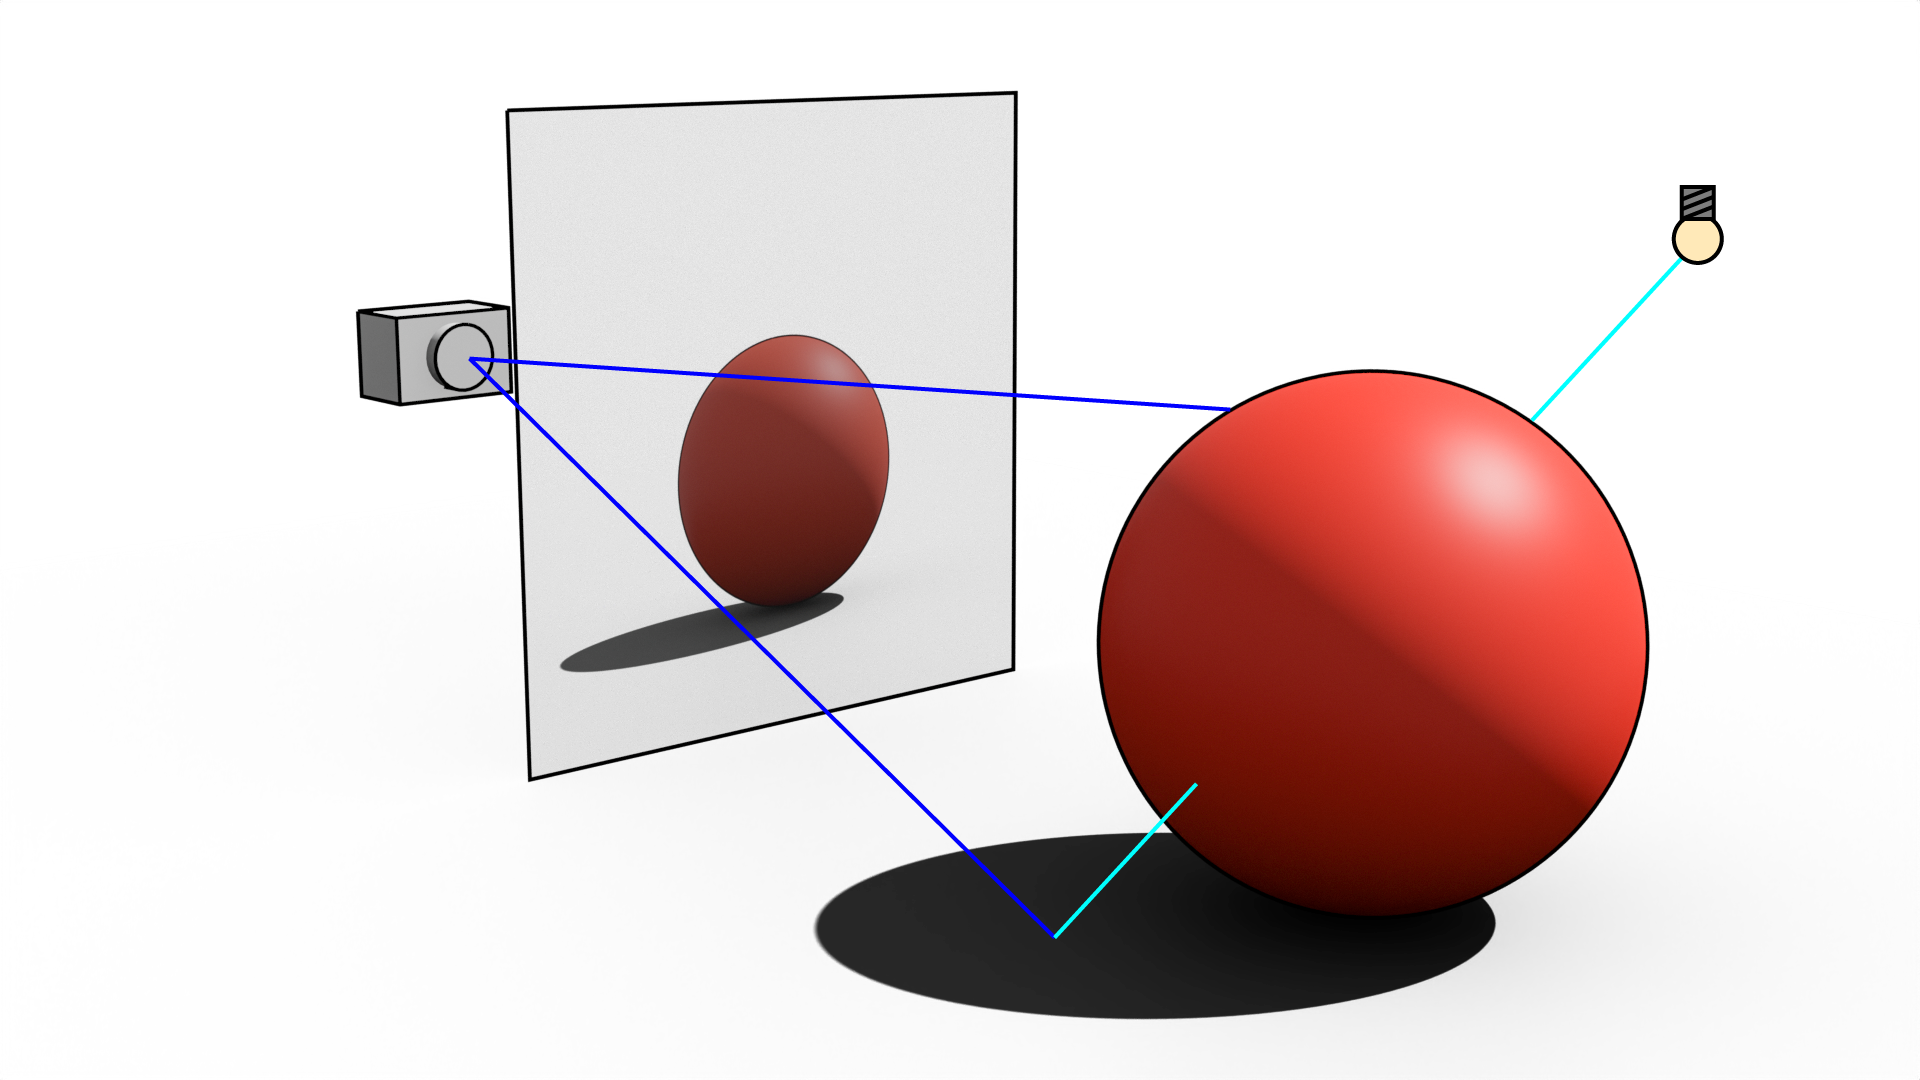
\includegraphics[width=\textwidth]{images/raymarching/raymarch_ai.png}
      \caption{Ray marching to produce an image}
      \label{fig:rmcast}
  \end{subfigure}
  %
  \begin{subfigure}[b]{0.45\textwidth}
      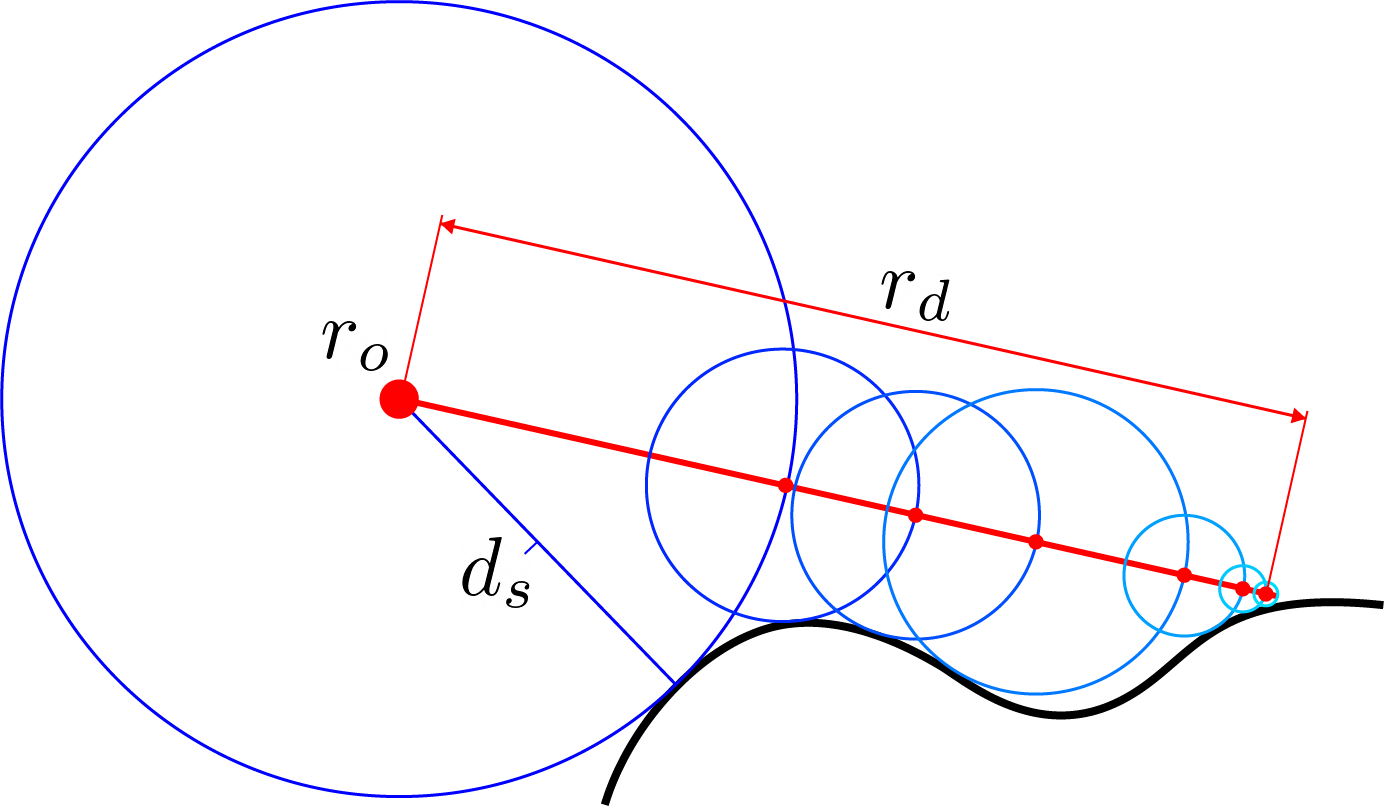
\includegraphics[width=\textwidth]{images/raymarching/algorithm_ai.png}
      \caption{Ray marching algorithm}
      \label{fig:rmalg}
  \end{subfigure}   
  %
  \caption{Ray marching. \subref{fig:rmcast} shows how each pixel of an image is coloured by casting a ray from the camera in the direction of the pixel and reading the surface of any defined geometry. 
  \subref{fig:rmalg} shows the process of a single ray marching towards a surface, given a an origin point and a direction as described in Algorithm \ref{alg:raymarch}.
  }\label{fig:raymarch}
\end{figure}

% Ray marching Algorithm
\begin{algorithm}
  \DontPrintSemicolon
  
  \KwData{\\
    \quad $r_o$ the origin of a ray.\;
    \quad $r_d$ the direction of a ray.\;
    \quad $MAX\_STEPS$ the maximum number of iterations.\;
    \quad $MAX\_DIST$ the maximum distance from the ray origin.\;
    \quad $SURF\_DIST$ the smallest distance from a surface before deciding not to step any further.\;
    \quad $SDF(p)$ given a point $p$ along the ray, return the distance to the nearest surface.\;
  }
  \KwResult{\\
    \quad $ d_o $ The distance from the ray origin along the ray path.
  }
  \Begin{
      $ d_o \longleftarrow 0 $\;
      $ d_s \longleftarrow \infty $\;
      \For{$ i < MAX\_STEPS $}
      {
          $ p \longleftarrow r_o + d_o \cdot r_d$\;
          $ d_s \longleftarrow SDF(p) $\;
          $ d_o \longleftarrow d_s + d_o $\;
          \If{$d_s < SURF\_DIST \textbf{ or } d_o > MAX\_DIST$}
          {
              break\;
          }
      }
  }
\caption{The ray marching algorithm}\label{alg:raymarch}
\end{algorithm}

\vskip 0.5em
Whilst less intuitive and approachable than mesh based rendering, there are active communities which strive to build interesting or complex geometry using these mathematical expressions in conjunction with ray marching. \textit{Shadertoy}, developed by \citet{quilez_shadertoy_2013}, is a web based platform that allows anyone to create and experiment with shader based geometry.
\vskip 0.5em
A significant advantage over mesh based rendering is the ability to render a 3D cross section of a 4D object with minimal effort. The SDF of a 4D object taken over three dimensional space will produce the SDF equivalent to the cross section of the same object in a given hyper plane along the \(w\) axis.
It is not novel to ray march over primitive 4D objects such as the hyper cube or hyper sphere. Often, primitive SDFs taken over $\mathbb{R}^3$ can be easily extended to $\mathbb{R}^4$; and this is the case for many of the SDFs developed by \citet{quilez_distance_nodate}. Other 4D geometry on the other hand would need to be derived from scratch. 

\section{Rotating a 4D Object}

In $\mathbb{R}^3$ there are three degrees of rotational freedom. As there are three axes, the method of rotating an object has commonly been considered as rotating about an axis. However, in $\mathbb{R}^4$ there are six degrees of rotational freedom, despite there only being four axes. Instead, rotation must be considered as a rotation about a plane formed by two axes. Therefore the six planes of rotation in $\mathbb{R}^4$ would be \(xy\), \(xz\), \(yz\), \(xw\), \(yw\) and \(zw\).

\subsection{The Problems with Rotation}

Rotating an object in $\mathbb{R}^2$ is somewhat trivial. Given a vector $v_{xy}$ rotating an angle $\theta$ about an origin point within the \(xy\) plane, the vector will follow a circular path dictated by the following 2D rotation matrix:
% 2D Rotation Matrix
\begin{equation}
    v_{xy}' = v_{xy}\begin{bmatrix}
      cos \theta & - sin \theta \\
      sin \theta & cos \theta
    \end{bmatrix},
\end{equation}
%
Rotating an object in a space greater than two dimensions immediately becomes a nontrivial problem due to its non-commutativity. In dimensions greater than $\mathbb{R}^2$, rotation matrices can be composed into a homogeneous rotation matrix. Multiplying a vector with a such a matrix will produce a rotated vector, but doing so will likely encounter gimbal lock. Gimbal lock occurs when rotating an object considers each plane of rotation as independent from one another. As a result, if a particular plane becomes parallel with another, a degree of rotation is lost and the vector being rotated will not change as expected.
\vskip 0.5em
Introducing the quaternion: The quaternion is an extension of the complex number system. A quaternion has 4 components: \(x\), \(y\) and \(z\) which describe the axis of rotation, and \(w\) which describes the amount of rotation. Quaternions do not suffer from gimbal lock and can be applied to each other to perform several rotations in series.
\vskip 0.5em
Quaternions have a problem: They consider rotations as a rotation about an axis. As discussed by \citet{bosch_lets_nodate}, axial rotations are not appropriate as a generalised method of rotation across dimensions. For example, you would not consider a 2D object rotating about the \(z\) axis. It makes far more sense to stay within $\mathbb{R}^2$ and rotate about the \(xy\) plane.

\subsection{Geometric Algebra and The Rotor}

Geometric Algebra, often referred to as Clifford Algebra, is a field of mathematics describing vector space. Vector space is populated by multivectors, graded by their vector components. Most notably, multivectors are defined by their associative, distributive and anti-commutative properties \citep{baker_maths_nodate}.
A grade zero multivector is a scalar number. a grade one multivector is just a vector. Grade two multivectors are known as bivectors, which build the foundation for the rotor. A trivector is a grade 3 multivector forming a parallelepiped from 3 vectors. Finally in $\mathbb{R}^4$ there is what is known as a pseudo-scalar.
\vskip 0.5em
A bivector $b_{ab}$ is made up of two vectors \(a\) and \(b\), and has, alongside its orientation in space defined by it's vector components, two important properties: The direction of rotation, from \(a\) to \(b\), and an area, dictated by the parallelogram formed by its two vector components as illustrated by \citet{slehar_clifford_2014}. A bivector in the reverse direction, i.e from \(b\) to \(a\) fulfills the anti-commutative property such that $b_{ba} = -b_{ab}$. 
% TODO: Wedge Product similar to Cross Product
\vskip 0.5em
As mentioned above, a rotation should be considered as a rotation about a plane. A bivector defines the plane for a vector to rotate about. As demonstrated by \citet{mathoma_geometric_2017}, a rotor can rotate a vector following the principle that a double reflection forms a rotation \citep{mathoma_geometric_2016-2}.
\vskip 0.5em
In a given vector space greater than $\mathbb{R}^2$, a multivector greater than grade zero can be projected onto the vector space basis blades. A basis blade is a the plane formed parallel to two perpendicular axes. The \(xy\) blade is often referred to as $e_{xy}$ or $e_{01}$. Therefore a bivector in $\mathbb{R}^3$ can be decomposed into three projections onto the $e_{xy}$, $e_{xz}$ and $e_{yz}$ planes; and a bivector in $\mathbb{R}^4$ can be decomposed into 6 elements.
\vskip 0.5em
It is possible to multiply multivectors using the geometric product; a combination of the inner and outer product. Multiplying a vector \(v\) by a rotor \(R\) and it's reverse \(R^\dagger\) will rotate vector about the bivector component of the rotor.
%
\begin{equation}
    v' = R v R^\dagger,
\end{equation}
%
The angle of rotation is dictated by a scalar component of the rotor, similar to the \(w\) component of a quaternion. 
As shown by \citep{bosch_code_nodate}, the quaternion and the 3D rotor are very similar in concept. The rotor, unlike the quaternion, has the advantage of not having to leave the dimension it belongs in order to rotate a vector, allowing it to be used in \(n\) dimensions.

\section{Interaction and Direct Manipulation}

\subsection{Methods of Interaction in 3D}

local, grab ball driven

global, swipe gestures (often multi-touch)

\citep{shoemake_arcball_1994}

\subsection{Methods of Interaction in 4D}

\citep{murata_interactive_2000}
\citep{kageyama_keyboard-based_2005}

\section{Teaching and Evaluation}

TODO: reiterate aims and questions

\citep{safrankova_van_2012}

%==================================================================================================================================
\chapter{Analysis and Requirements}

self defined project with the goal of teaching people about abstract mathematical concepts

\section{Problem Specification}

teach people, and develop something suited to teaching people

\section{Limitations}

time to develop

time per user to experiment\\
 - quantity of quality

\section{Prioritisation Using MoSCoW}

explanation of MoSCoW

\subsection*{Must Have}

be able to render multiple 4D shapes

multiple extensions to a 3d cross section of 4d space

create a tutorial video to teach and explain 4d
 - must cover the geometry
 - must cover the rotation

\subsection*{Should Have}

be able to interact with them in 4D directly

multiple tests to evaluate a persons understanding

\subsection*{Could Have}

multiple methods of direct interaction/manipulation

%===

What is the problem that you want to solve, and how did you arrive at it?

%==================================================================================================================================
\chapter{Design}

\section{Tutorial}

requirements for teaching

 - explain 4D space, why it cannot be visualised
 - explain 4D rotation in relation to 2D and 3D rotation

\section{Experiment}

requirements for testing

 - be able to understand the shapes
 - be able to interpret the rotation of a shapes
 - be able to manipulate a shape

%==================================================================================================================================
\chapter{Implementation}

\section{Building 4D Objects With Ray Marching}

shapes defined with signed distance functions

relative to the camera - slice is based on W coordinate of camera based

algorithm

\subsection{Derivation of 4D Shapes}


\section{Extending 3 Dimensional Cross Sections - Representing 4D Objects}

timeline: simple - ellyptical version
 - ellypitcal adds more information, but not as intuitive as straight line\\
onionskin - similar to timeline, but not very intuitive for users unfamiliar with 4D\\
multi-view: polyvision\\
abstraction of 4D rotation using 3D rotation - does not extend well to n dimensions unlike all other propersitions

\section{Rotation of a 4D Vector}

\citep{bosch_4d_2011}
\citep{bosch_code_nodate}

initial manual derivation

sympy and galgebra

equations

\section{Methods of Rotation}

\subsection{Swipe Based Input - Rotation About The Global Axes}

intuitive\\
does not define "how rotated" 4D axes are relative to the local coordinates of the shape

\subsection{4D Grab Ball - Rotation About The Local Axes}

idea\\
progress\\
why it failed

\section{Texturing Ray Marched Objects}

normal based projection

\section{Building the Experiment}

\subsection{}

\subsection{Data Collection}

SimpleJSON

Email - challenges\\
Copy \& Paste - challenges

%==================================================================================================================================
\chapter{Evaluation} 

\section{Aims} 

\section{Experimental Design}

\subsection{Preliminary Research}

what is the best way to explain concepts\\
try teach some friends the basics and see what explanations work best

the best ways to teach people about geometry\\
 - reference that paper about 5 stages or something

between users experiment
 - test user with every representation

\subsection{Repeated Preliminary Experiments}

build system\\
test it\\
improvements\\

Need to provide clear explanations of concepts early on

provide time to play with object before tests to learn controls and behaviour

\subsection{Tasks and Parameters}

shape match\\
 - all shapes\\
 - diffuse texture - patterns give it away\\
rotation match\\
 - not diffuse texture and no sphere - no surface imperfections and can be impossible to tell if certain rotations occuring\\
 - 1-2 4D rotations and occasionally 3d rotations\\
pose match\\
 - randomly oriented match shape

random order of representations

\subsection{Limitations}

\section{Results}


%==================================================================================================================================
\chapter{Conclusion}    
Summarise the whole project for a lazy reader who didn't read the rest (e.g. a prize-awarding committee).
\section{Guidance}
\begin{itemize}
    \item
        Summarise briefly and fairly.
    \item
        You should be addressing the general problem you introduced in the
        Introduction.        
    \item
        Include summary of concrete results (``the new compiler ran 2x
        faster'')
    \item
        Indicate what future work could be done, but remember: \textbf{you
        won't get credit for things you haven't done}.
\end{itemize}

%==================================================================================================================================
%
% 
%==================================================================================================================================
%  APPENDICES  

\begin{appendices}

\chapter{Appendices}

Typical inclusions in the appendices are:

\begin{itemize}
\item
  Copies of ethics approvals (required if obtained)
\item
  Copies of questionnaires etc. used to gather data from subjects.
\item
  Extensive tables or figures that are too bulky to fit in the main body of
  the report, particularly ones that are repetitive and summarised in the body.

\item Outline of the source code (e.g. directory structure), or other architecture documentation like class diagrams.

\item User manuals, and any guides to starting/running the software.

\end{itemize}

\textbf{Don't include your source code in the appendices}. It will be
submitted separately.

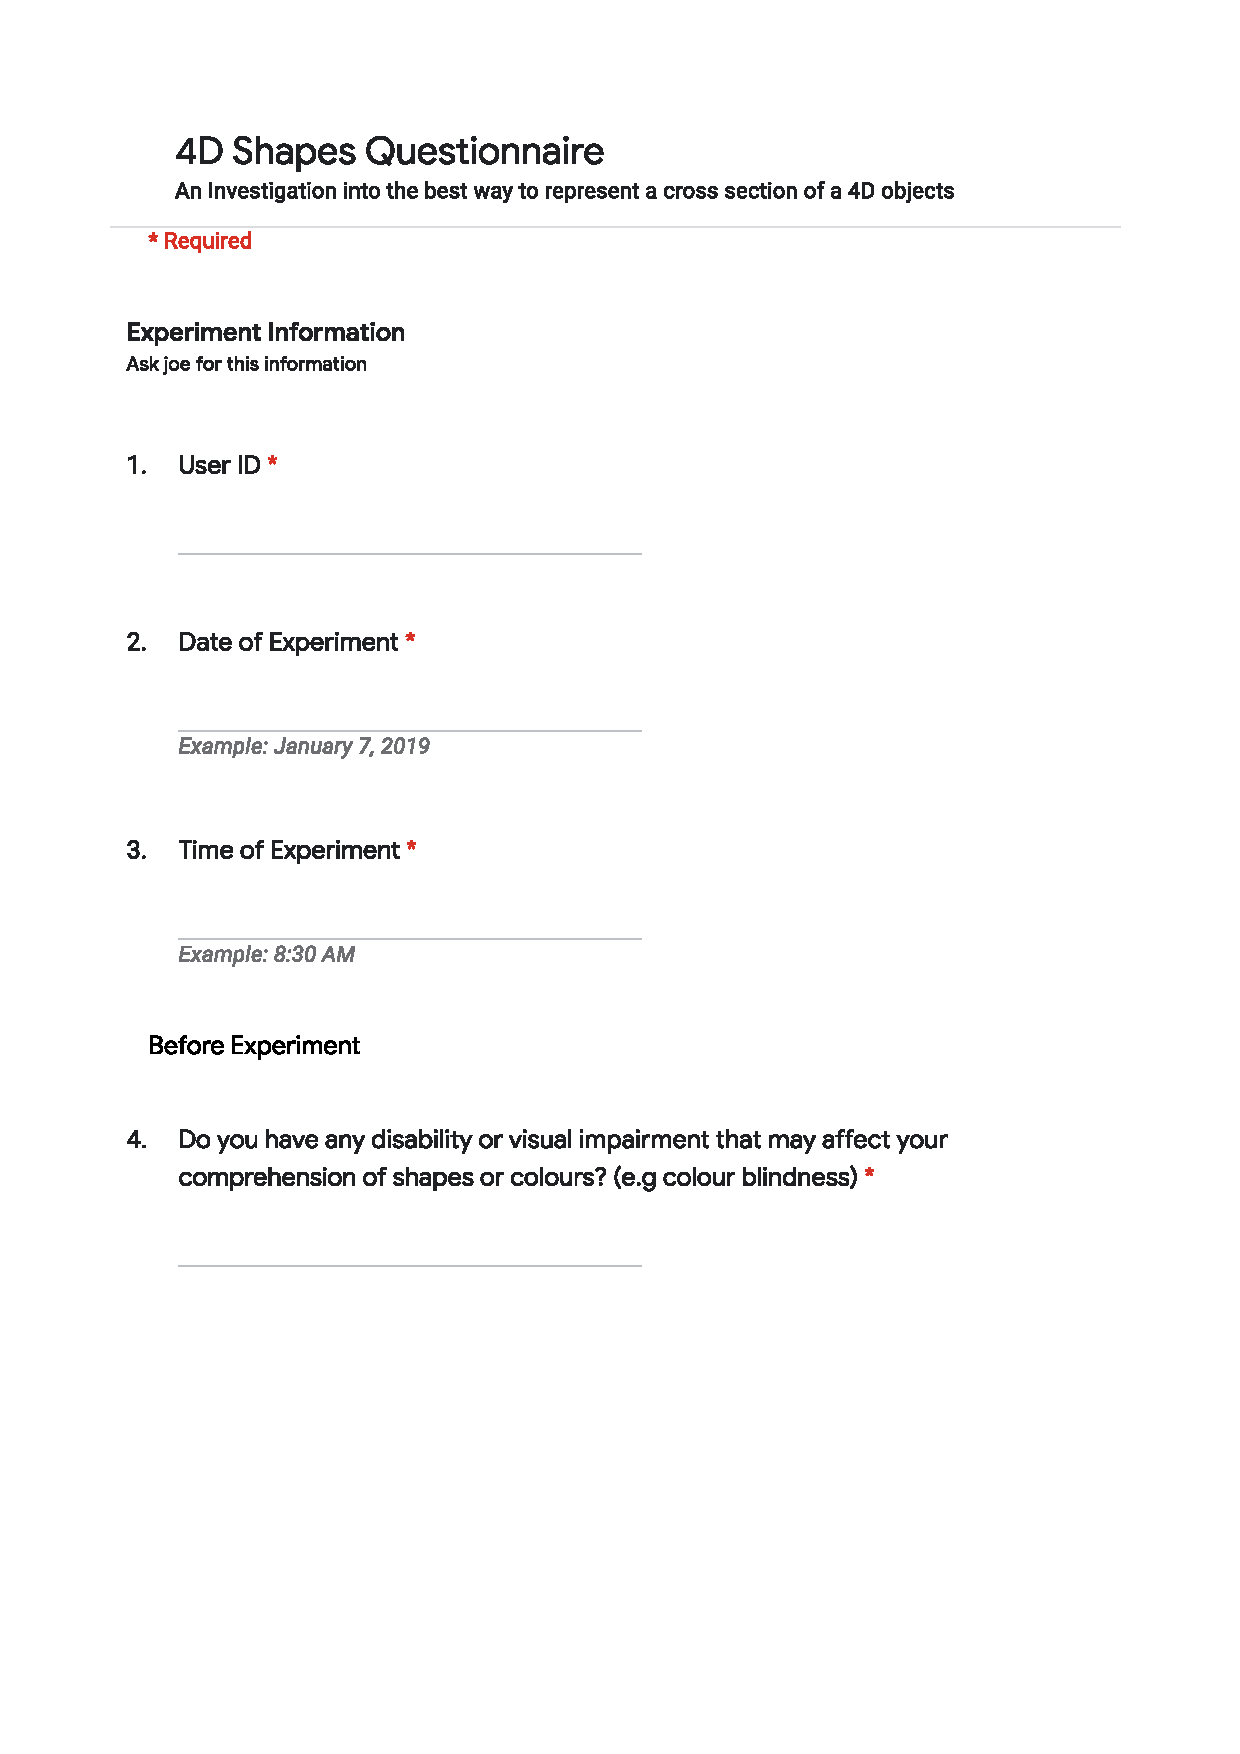
\includepdf[width=1.1\linewidth, pages={1-4}]{images/4d_shapes_questionnaire.pdf}

\end{appendices}

%==================================================================================================================================
%   BIBLIOGRAPHY   

% The bibliography style is abbrvnat
% The bibliography always appears last, after the appendices.

\bibliographystyle{abbrvnat}

\bibliography{l4proj}

\end{document}
